%%%%%%%%%%%%%%%%%%%%%%%%%%%%%%%%%%%%%%%%%%%%%%%%%%%%%%%%%%%%%%%%%
% MUW Presentation
% LaTeX Template
% Version 1.0 (27/12/2016)
%
% License:
% CC BY-NC-SA 4.0 (http://creativecommons.org/licenses/by-nc-sa/3.0/)
%
% Created by:
% Nicolas Ballarini, CeMSIIS, Medical University of Vienna
% nicoballarini@gmail.com
% http://statistics.msi.meduniwien.ac.at/
%
% Customized for UAH by:
% David F. Barrero, Departamento de Automática, UAH
%%%%%%%%%%%%%%%%%%%%%%%%%%%%%%%%%%%%%%%%%%%%%%%%%%%%%%%%%%%%%%%%%

\documentclass[10pt,compress]{beamer} % Change 10pt to make fonts of a different size
\mode<presentation>

\usepackage[spanish]{babel}
\usepackage{fontspec}
\usepackage{tikz}
\usepackage{etoolbox}
\usepackage{xcolor}
\usepackage{xstring}
\usepackage{listings}
\usepackage{tikz}
\usetikzlibrary{matrix,chains,positioning,decorations.pathreplacing,arrows,shapes}

\usetheme{UAH}
\usecolortheme{UAH}
\setbeamertemplate{navigation symbols}{} 
\setbeamertemplate{caption}[numbered]

%%%%%%%%%%%%%%%%%%%%%%%%%%%%%%%%%%%%%%%%%%%%%%%%%%%%%%%%%%%%%%%%%
%% Presentation Info
\title[Scientific Programming]{Scientific Programming in Python}
\author{\asignatura\\\carrera}
\institute{}
\date{Departamento de Automática}
%%%%%%%%%%%%%%%%%%%%%%%%%%%%%%%%%%%%%%%%%%%%%%%%%%%%%%%%%%%%%%%%%


%%%%%%%%%%%%%%%%%%%%%%%%%%%%%%%%%%%%%%%%%%%%%%%%%%%%%%%%%%%%%%%%%
%% Descomentar para habilitar barra de navegación superior
\setNavigation
%%%%%%%%%%%%%%%%%%%%%%%%%%%%%%%%%%%%%%%%%%%%%%%%%%%%%%%%%%%%%%%%%

%%%%%%%%%%%%%%%%%%%%%%%%%%%%%%%%%%%%%%%%%%%%%%%%%%%%%%%%%%%%%%%%%
%% Configuración de logotipos en portada
%% Opacidad de los logotipos
\newcommand{\opacidad}{1}
%% Descomentar para habilitar logotipo en pié de página de portada
\renewcommand{\logoUno}{Images/isg.png}
%% Descomentar para habilitar logotipo en pié de página de portada
%\renewcommand{\logoDos}{Images/CCLogo.png}
%% Descomentar para habilitar logotipo en pié de página de portada
%\renewcommand{\logoTres}{Images/ALogo.png}
%% Descomentar para habilitar logotipo en pié de página de portada
%\renewcommand{\logoCuatro}{Images/ELogo.png}
%%%%%%%%%%%%%%%%%%%%%%%%%%%%%%%%%%%%%%%%%%%%%%%%%%%%%%%%%%%%%%%%%

%%%%%%%%%%%%%%%%%%%%%%%%%%%%%%%%%%%%%%%%%%%%%%%%%%%%%%%%%%%%%%%%%
%% FOOTLINE
%% Comment/Uncomment the following blocks to modify the footline
%% content in the body slides. 


%% Option A: Title and institute
\footlineA
%% Option B: Author and institute
%\footlineB
%% Option C: Title, Author and institute
%\footlineC
%%%%%%%%%%%%%%%%%%%%%%%%%%%%%%%%%%%%%%%%%%%%%%%%%%%%%%%%%%%%%%%%%

\begin{document}

%%%%%%%%%%%%%%%%%%%%%%%%%%%%%%%%%%%%%%%%%%%%%%%%%%%%%%%%%%%%%%%%%
% Use this block for a blue title slide with modified footline
{\titlepageBlue
    \begin{frame}
        \titlepage
    \end{frame}
}

\begin{frame}[plain]{}
	\begin{block}{Objectives}
		\begin{enumerate}
		\item Motivate the need of efficient matrix representations.
		\item Introduce some Python scientific tools.
		\item Handle data representations in Python.
		\item Basic data visualization with Python.
		\item Provide a background for scientific programming.
		\end{enumerate}
	\end{block}

   \begin{block}{Bibliography}
       Jake VanderPlas. \textit{Python Data Science Handbook}. Chapters 1, 2, 3 and 4. O'Reilly. \href{https://jakevdp.github.io/PythonDataScienceHandbook/}{(Link)}.
   \end{block}

\end{frame}

{
\disableNavigation{white}
\begin{frame}[shrink]{Table of Contents}
 \frametitle{Table of Contents}
 \tableofcontents
  % You might wish to add the option [pausesections]
\end{frame}
}

\section{Overview}

\subsection{Data Science}

\begin{frame}{Overview}{Data Science}
	\begin{figure}
		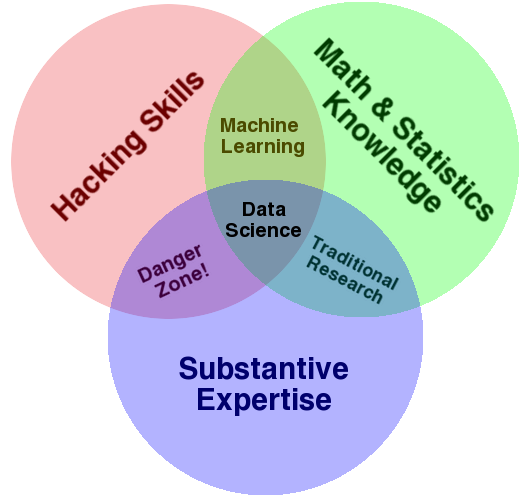
\includegraphics[scale=0.35]{figs/Data_Science_VD.png}	
	\end{figure}				
\end{frame}

\subsection{The data scientist toolkit}

\begin{frame}{Data Science}{The data scientist tookit (I)}
	Data science is about manipulating data
	\begin{itemize}
		\item Need of specialized tools
		\item Two main languajes: R and Python
	\end{itemize}
	Python is a general purpose programming language
	\begin{itemize}
		\item Easy integration 
		\item Huge ecosystem of packages and tools
	\end{itemize}
	Need of data-oriented tools
	\begin{itemize}
		\item Features provided by third-party tools
	\end{itemize}

\end{frame}

\begin{frame}{Data Science}{The data scientist tookit (II)}
   \begin{tabular}{cll}\hline
       \textbf{Tool}& \textbf{Type} & \textbf{Description}\\ \hline
	   \texttt{iPython} & Software & Advaced Python interpreter \\
	   \texttt{Jupiter} & Software & Python notebooks (Python interpreter) \\
	   \texttt{Numpy}   & Package  & Efficient array operations \\
	   \texttt{Pandas}  & Package  & Dataframe support \\
	   \texttt{Matplotlib} & Package & Data visualization \\
	   \texttt{Seaborn} & Package & Data visualization with dataframes \\
	   \texttt{Scikit-learn} & Package & AI/ML package for Python \\
	   \hline
   \end{tabular}
\end{frame}

\subsection{Anaconda}
\begin{frame}{Data Science}{Anaconda}
    \begin{columns}
 	   \column{.6\textwidth}
   All those tools are packaged in \texttt{Anaconda}
   \begin{itemize}
   		\item Python distribution for Data Science
	\end{itemize}

	Anaconda provides \texttt{Spyder}
	\begin{itemize}
		\item Python IDE designed for Data Science
	\end{itemize}

	Other tools provided by Anaconda
	\begin{itemize}
		\item Conda: Packages management tool
		\item TensorFlow: Deep Learning 
		\item Many others
	\end{itemize}

 		\column{.4\textwidth}
			
\includegraphics[width=0.6\textwidth]{figs/Anaconda_Logo.png} \\\bigskip
			
\includegraphics[width=0.6\textwidth]{figs/spyder.png}	
			%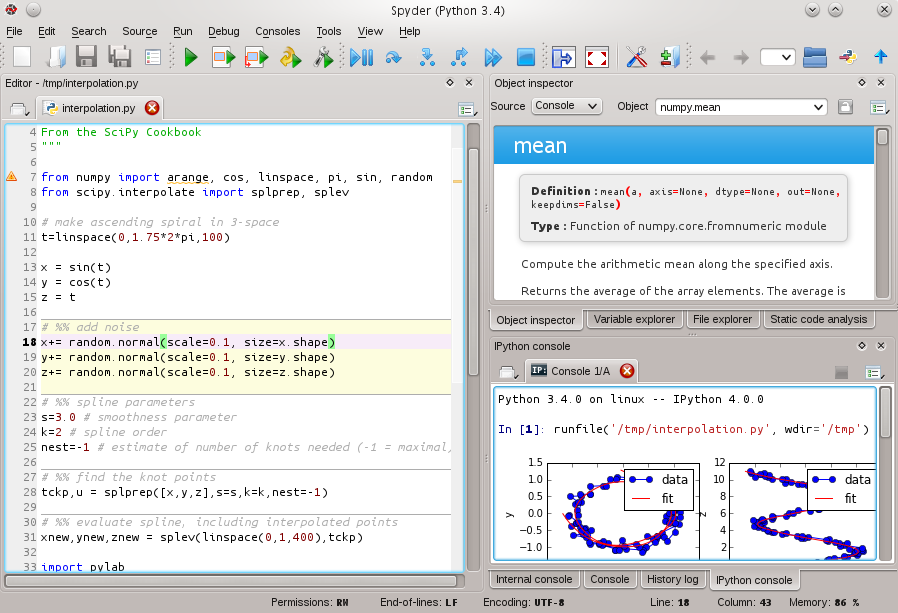
\includegraphics[width=0.6\textwidth]{figs/spyder-ide.png}	
	\end{columns}
\end{frame}

\subsection{Python IDEs for Data Science}
\begin{frame}{Data Science}{Python IDEs for Data Science (I)}
    \begin{columns}[t]
 	   \column{.25\textwidth}
	   \centering \textbf{iPython}\\
	   iPython = Interactive Python
   		\begin{itemize}
		\item Extended funcionality
		\item Enhanced UI
		\item External editor
		\end{itemize}

		Running iPython:\\
		\texttt{\$ ipython}

 	   \column{.25\textwidth}
	   \centering \textbf{Jupyter}\\
		Python notebooks
	\begin{itemize}
		\item Web-based IDE
		\item Documentation
		\item Integration with GitHub
		\item Uses iPython
	\end{itemize}

		Running Jupyter:\\
		\texttt{\$ jupyter notebook}

		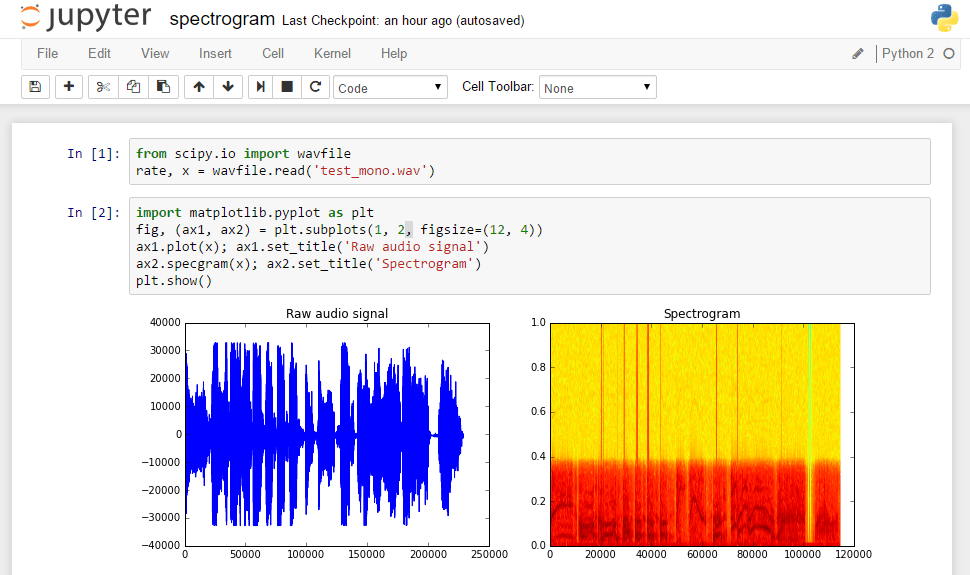
\includegraphics[width=0.8\textwidth]{figs/jupyter.png}	

 	\column{.25\textwidth}
	   \centering \textbf{Rodeo}\\
		Python version of RStudio
		\begin{itemize}
			\item Good for R developers
			\item Not included in Anaconda
			\item Uses iPython
		\end{itemize}
        
        \bigskip

		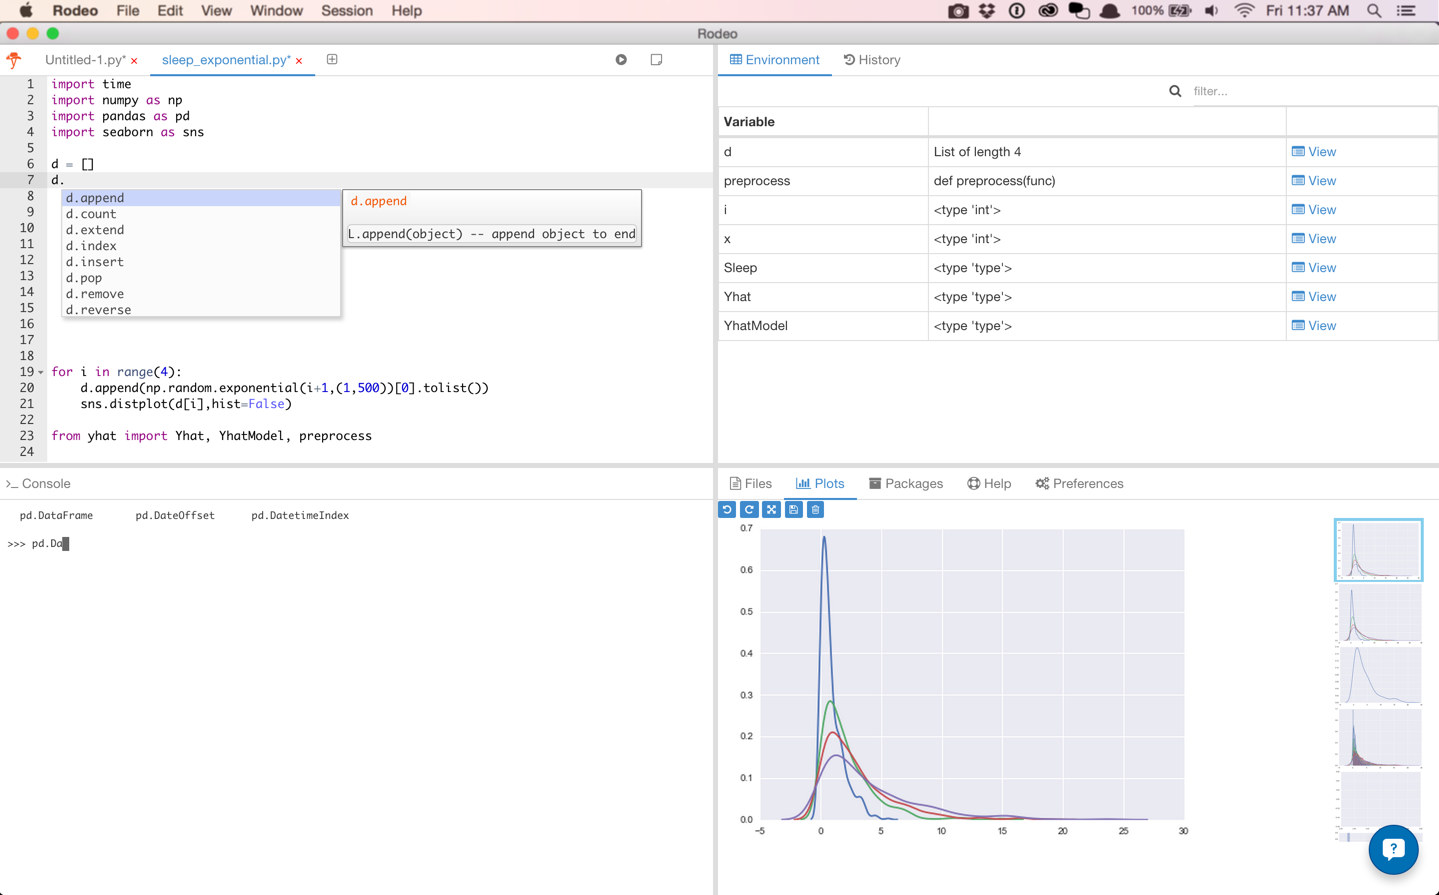
\includegraphics[width=0.8\textwidth]{figs/rodeo.png}	

 	\column{.25\textwidth}
	   \centering \textbf{Spyder}\\
		Matlab-like IDE

        \bigskip

		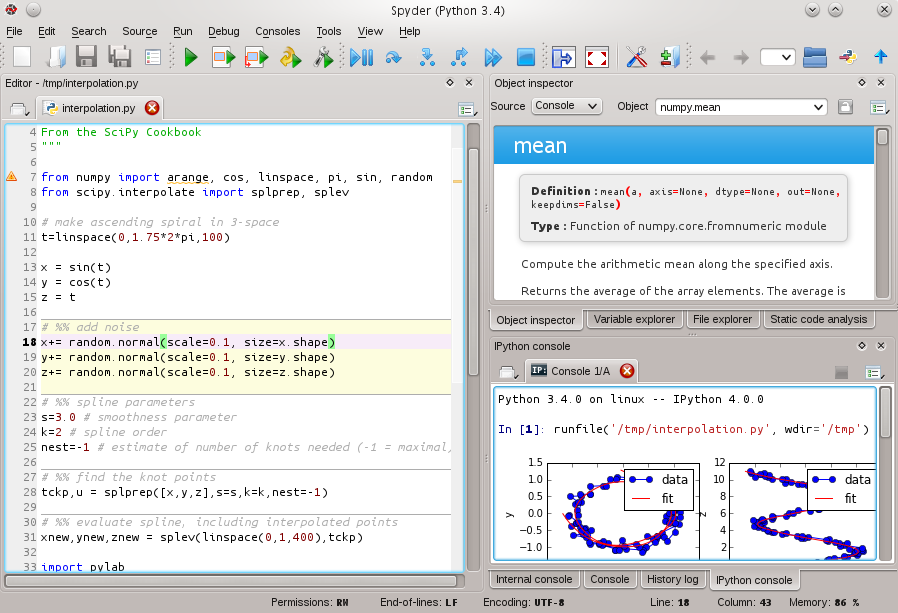
\includegraphics[width=0.8\textwidth]{figs/spyder-ide.png}	

	\end{columns}
\end{frame}

\begin{frame}{Data Science}{Python IDEs for Data Science (II)}
    \begin{block}{Exercises}
		Write a Python script that shows the multiplication table of the number 5. Write the script using each one of the following environments:
   		\begin{enumerate}
   		\item iPython + text editor of your choice.
		\item Jupiter. 
            \begin{itemize}
                \item Bonus track: Publish the notebook in GitHub.
            \end{itemize}
		\item Spyder.
		\item Rodeo.
		\end{enumerate}
	\end{block}
\end{frame}

\section{Basics}
\begin{frame}{iPython}{Basics (I)}
    In regular Python ...
    \begin{itemize}
        \item most objects come with a docstring attribute
        \item docstring accesible thorugh \texttt{help()}
    \end{itemize}
    iPython provides `\texttt{?}', a shortcut to \texttt{help()}
    \begin{itemize}
        \item \texttt{len?}, \texttt{list?}, \texttt{list.append?}
        \item Try to type just `\texttt{?}'
    \end{itemize}
    Easy access to source code with `\texttt{??}'
    \begin{itemize}
        \item Does not work with most buildin functions!
    \end{itemize}
\end{frame}

\begin{frame}{iPython}{Basics (II)}
    Press \texttt{<tab>} to complete almost everything
    \begin{itemize}
        \item Object contents\\
	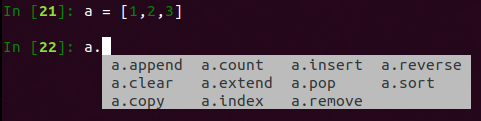
\includegraphics[width=0.45\textwidth]{figs/tab.png} 
        \item Packages\\
	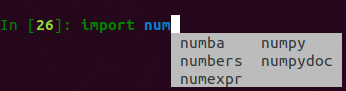
\includegraphics[width=0.36\textwidth]{figs/tab2.png}	
        \item Wildcards\\
	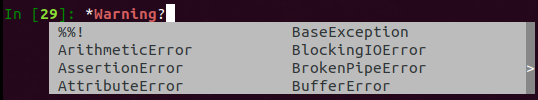
\includegraphics[width=0.45\textwidth]{figs/tab3.png}	
    \end{itemize}
\end{frame}

\begin{frame}{iPython}{Basics (III): Keyboard shortcuts}
    \footnotesize{
        Navigation\\
        \begin{tabular}{ll}\hline
       \textbf{Keystroke} &  \textbf{Action}\\ \hline
	   \texttt{Ctrl-a} & Move cursor to the beginning of the line  \\
	   \texttt{Ctrl-e} & Move cursor to the end of the line  \\
	   \texttt{Ctrl-b} & Move cursor back one character  \\
	   \texttt{Ctrl-f} & Move cursor forward one character  \\\hline
        \end{tabular}

    \bigskip
     History\\
       \begin{tabular}{ll}\hline
       \textbf{Keystroke} &  \textbf{Action}\\ \hline
       \texttt{Ctrl-p ($\uparrow$)} & Previous command  \\
       \texttt{Ctrl-n ($\downarrow$)} & Next command  \\
	   \texttt{Ctrl-r} & Reverse-search  \\\hline
    \end{tabular}

    \bigskip
        Text entry\\
        \begin{tabular}{ll}\hline
       \textbf{Keystroke} &  \textbf{Action}\\ \hline
	   \texttt{Ctrl-d} & Delete next character in line  \\
	   \texttt{Ctrl-k} & Cut text from cursor to end of line  \\
	   \texttt{Ctrl-u} & Cut text from beginning of line to cursor  \\
       \texttt{Ctrl-y} & Yank (paste) previously cut text  \\\hline
       \end{tabular}
   }
\end{frame}

\subsection{Magic commands}
\begin{frame}{iPython}{iPython magic commands}
	Magic commands: iPython extension of Python syntax
	\begin{itemize}
	\item Not valid in regular Python
	\item Provides handly features
	\item Widely used in DS and ML
	\end{itemize}
	Two flavours
	\begin{itemize}
	\item \% prefix: Line magics - single line
	\item \%\% prefix: Cell magics - several lines
	\end{itemize}
	Help available
	\begin{itemize}
		\item \texttt{\%magic}: Magic commands
		\item \texttt{\%lsmagic}: List of magic commands
	\end{itemize}
\end{frame}

\subsection{Pasting code blocks}
\begin{frame}[fragile]{iPython}{Pasting code blocks: \texttt{\%paste} and \texttt{\%cpaste}}
    \begin{columns}
 	   \column{.5\textwidth}
	   Pasting code in Python is troublesome
		\begin{itemize}
			\item \texttt{\%paste}: Paste one time
			\item \texttt{\%\%cpaste}: Paste several times
		\end{itemize}
 	   \column{.5\textwidth}
	       %\begin{block}{}
		   %    \vspace{-0.2cm}
		   %    \lstinputlisting{code/donothing.py}
		   %    \vspace{-0.2cm}
		   %\end{block}
	   \begin{exampleblock}{}
	   \vspace{-0.2cm}
	   \begin{verbatim}
def donothing(x):
    return x
	   \end{verbatim}
	   \vspace{-0.2cm}
	   \end{exampleblock}

	   \vspace{-0.2cm}
	\end{columns}

	\footnotesize{
    \begin{columns}
 	   \column{.4\textwidth}
		 \begin{exampleblock}{\%paste}
	   \vspace{-0.2cm}
	   \begin{verbatim}
In [20]: %paste
   def donothing(x):
 	  return x

## -- End pasted text --
\end{verbatim}
	   \vspace{-0.2cm}
	   \end{exampleblock}

	   \vspace{-0.2cm}

 	   \column{.6\textwidth}

	 	\begin{exampleblock}{\%cpaste}
	   \vspace{-0.2cm}
	   \begin{verbatim}
In [25]: %cpaste
Pasting code; enter '--' alone on the line
to stop or use Ctrl-D.
:       def donothing(x):
            return x:
:--
	   \end{verbatim}
	   \vspace{-0.2cm}
	   \end{exampleblock}
	   \end{columns}
	   }
\end{frame}

\subsection{Running external code}
\begin{frame}[fragile]{iPython}{Running external code: \texttt{\%run} and \texttt{\%timeit}}
    \begin{columns}
 	   \column{.4\textwidth}
	   \texttt{\%run}: Execute script
		\begin{itemize}
			\item Many optional arguments
			\item Checkout \texttt{\%run?}
		\end{itemize}
		\footnotesize{
	   \begin{exampleblock}{}
	   \vspace{-0.2cm}
	   \begin{verbatim}
In [40]: %run donothing.py

In [41]: donothing(10)
Out[41]: 10
	   \end{verbatim}
	   \vspace{-0.2cm}
	   \end{exampleblock}
		}

 	   \column{.6\textwidth}
	   \texttt{\%timeit}: Computes execution time
		\begin{itemize}
			\item Executes a single line
			\item Automatic adjustment of runs
			\item Shows basic statistics
		\end{itemize}

		\footnotesize{
	   \begin{exampleblock}{}
	   \vspace{-0.2cm}
	   \begin{verbatim}
In [33]: %timeit [n ** 2 for n in range(200)]
71.6 µs ± 1.84 µs per loop 
(mean ± std. dev. of 7 runs, 10000 loops each)

In [34]: %timeit [n ** 2 for n in range(2000)]
753 µs ± 16.2 µs per loop 
(mean ± std. dev. of 7 runs, 1000 loops each)
\end{verbatim}
	   \vspace{-0.2cm}
	   \end{exampleblock}
		}

		\normalsize{
	   \texttt{\%\%timeit}: Several lines\\
	   }
	\end{columns}

\end{frame}

\subsection{Input and output history}
\begin{frame}[fragile]{iPython}{Input and output history (I)}
	\begin{columns}
 	   \column{.6\textwidth}
	iPython stores its history as objects
	\begin{itemize}
		\item \texttt{In}: Input commands
			\begin{itemize}
			\item List storing commands
			\end{itemize}
		\item \texttt{Out}: Commands output
			\begin{itemize}
			\item Dictionary storing outputs
			\item Not all commands have outputs
			\end{itemize}
	\end{itemize}

	\vspace{-0.2cm}

 	   \column{.4\textwidth}
	\begin{exampleblock}{}
In [1]: import math

In [2]: math.sin(2)

Out[2]: 0.9092974268256817

In [3]: math.cos(2)

Out[3]: -0.4161468365471424

In [4]: Out[2] ** 2 + Out[3] ** 2

Out[4]: 1.0
	\end{exampleblock}
	\end{columns}
\end{frame}

\begin{frame}{iPython}{Input and output history (II)}
	Fast access to history: Underscore (\_)
	\begin{itemize}
		\item Variable containing the last output
		\item Example: \texttt{print(\_)}
	\end{itemize}
	Double and triple underscores
	\begin{itemize}
		\item Example: \texttt{print(\_\_)}
		\item Example: \texttt{print(\_\_\_)}
	\end{itemize}
	Trick: Shortcut to access ($\_n$)
	\begin{itemize}
		\item Out[n] = \_n, with n=number
		\item Example: \texttt{print(\_2)}
	\end{itemize}
	Magic command to show history
		\begin{itemize}
		\item \texttt{\%history}
		\end{itemize}
	Supressing command output (\texttt{;})
		\begin{itemize}
		\item Example: \texttt{4 * 2;}
		\end{itemize}
\end{frame}

\subsection{iPython shell commands}
\begin{frame}{iPython}{iPython shell commands}
	iPython provides easy interaction with the shell
	\begin{itemize}
		\item Execution of shell commands from iPython
		\item Use prefix `\texttt{!}'
		\item Example: \texttt{!ls}, \texttt{!pwd}
	\end{itemize}
	Save shell output in Python variables
	\begin{itemize}
		\item Example: \texttt{files = !ls}
	\end{itemize}
	Use Python variables in shell
	\begin{itemize}
		\item Example: \texttt{!echo \{files\}}
	\end{itemize}
\end{frame}

\subsection{Automagic}

\begin{frame}[fragile]{iPython}{Automagic}
	\begin{columns}
 	   \column{.4\textwidth}
	Problems with some shell commands
	\begin{exampleblock}{}
In [23]: !pwd

/repositorios/pythonCourse


In [24]: !cd ..


In [25]: !pwd

/repositorios/pythonCourse
	\end{exampleblock}
	Some magic commands here to help
	\begin{itemize}
		\item \texttt{\%cd}, \texttt{\%ls}, \texttt{\%mkdir}, \texttt{\%pwd}, ...
	\end{itemize}

 	   \column{.4\textwidth}
	Those magics are regularly used ...
	\begin{itemize}
		\item ... so common that \% is no longer required (automagic)
		\item Working with iPython is almost like working with a Unix-like shell
	\end{itemize}

	\begin{block}{Automagic commands}
\texttt{cat}, \texttt{cp}, \texttt{env}, \texttt{ls}, \texttt{man}, \texttt{mkdir}, \texttt{more}, \texttt{mb}, \texttt{pwd}, \texttt{rm} and \texttt{rmdir}
	\end{block}

	\end{columns}

\end{frame}

\section{Numpy}
\section{Pandas}
\section{Matplotlib}
\section{Seaborn}



%\begin{frame}[plain]{Solved exercise. Serializando objetos \texttt{Parcela}}{}
%	\vspace{-0.4cm}
  %  \begin{columns}
 %	   \column{0.8\textwidth}
%			\begin{block}{\footnotesize{tasaparcela\_pickle.py}}
%			\vspace{-0.2cm} 
%				\lstinputlisting[basicstyle=\ttfamily\scriptsize]{code/tasaparcela_pickle.py} % contar elementos
%			\vspace{-0.2cm} 
%			\end{block}
%	\end{columns}
	
%\end{frame}


\end{document}
